\label{sec:evaluation}

We perform all of our evaluations on a quiescent 8-core system (dual processor with 4 cores), with 8GB of RAM. Each processor is a 4-core 64-bit Intel Xeon, running at 2.33 Ghz with a 4MB L2 cache. For compatibility reasons, we compiled all applications to a 32-bit target using the GCC compiler. All performance data is the average of ten runs, excluding the maximum and minimum values.

The evaluation answers the following questions:

\begin{itemize}
\item How effective is \sheriffdetect{} at finding false sharing and guiding programmers to their resolution? (Section~\ref{sec:effecteval})
\item What is \sheriffdetect{}'s performance overhead? (Section~\ref{sec:results-runtime-overhead})
\item How sensitive is \sheriffdetect{} to different sampling rate? (Section~\ref{sec:results-sampling-overhead}) 
\item How effective does \sheriffprotect{} mitigate false sharing? (Section~\ref{})
\end{itemize}

\subsection{\sheriffdetect{} Effectiveness}

\label{sec:effecteval}

This section evaluates whether \sheriffdetect{} can be used to find false sharing problems, both in synthetic test cases and in actual applications.

We developed a range of microbenchmarks that exemplify different situations related to false sharing. We evaluate these benchmarks on both \SheriffDetect{} and Intel's Performance Tuning Utility(PTU v3.2), the previous state-of-the-art work of false sharing detection. 

Detection results are shown in Table~\ref{table:microbenchmarks}. \sheriffdetect{} only reports those false sharing instances that can possibly affect the performance, while correctly ignores those cases without performance impact.
PTU has false alarms/positives.  It does not track those pattern of accesses, which reports false positives for those non-interleaved accesses. Also, PTU does not track memory deallocations, thus it can not filter out those pseudo false sharing caused by memory reuse. \sheriffdetect{} avoids all of these problems and reports false sharing problems correctly. 


\begin{table}
\centering
\resizebox{\columnwidth}{!}{
\begin{tabular}{l|l|l|l}
\hline
{\bf \small Microbenchmark} & {\bf \small Perf Sensitive } & {\bf \small \sheriffdetect{} } & {\bf \small PTU } \\
\hline

\small \textbf{False Sharing (adjacent objects)} & YES & \cmark{} & \cmark{} \\
\small \textbf{False Sharing (same object)} & YES & \cmark{} & \cmark{} \\
\hline
\small \textbf{True Sharing} & NO & & \\
\small \textbf{Non-interleaved False Sharing} & NO & & \xmark{}\\
\small \textbf{Heap Reuse(no sharing)} & NO & & \xmark{}\\
\hline
\end{tabular}
}
\caption{False sharing detection results using PTU and \sheriffdetect{}. \sheriffdetect{} correctly reports only actual false sharing instances, with a performance impact;
\cmark{} indicates a correct report and \xmark{} indicates a false alarm. 
\label{table:microbenchmarks}}
\end{table}

We further evaluate \SheriffDetect{} and PTU on two widely-used benchmarks suites, Phoenix~\cite{phoenix-hpca} and PARSEC~\cite{parsec}. We use the simlarge inputs for all applications of PARSEC. For Phoenix, we chose available parameters that allow the programs to run as long as possible. As of this writing, we were unable to successfully compile \texttt{raytrace} and \texttt{vips}, and \sheriff{} is
currently unable to run \texttt{x264}, \texttt{bodytrack},
and \texttt{facesim}. \texttt{Freqmine} currently can not support \pthreads{}. Thus, those benchmarks are excluded here. 
 
\begin{table}
\centering
\begin{tabular}{l|r|r}
\hline
{\bf \small Benchmark} & {\bf \small PTU} & {\bf \small \sheriffdetect{}}\\
 & {\# Lines} & {\# Objects}\\
\hline
\small \textbf{kmeans} & 1916 &  2 \\
\small \textbf{linear\_regression} & 5 & 1 \\
\small \textbf{matrix\_multiply} & 468 & 0\\
\small \textbf{pca} & 45 & 0 \\
\small \textbf{reverseindex} & N/A & 5 \\
\small \textbf{word\_count} & 4 & 3\\
\hline
\small \textbf{canneal} & 1 & 1 \\
\small \textbf{fluidanimate} & 3 & 1 \\
\small \textbf{streamcluster} & 9 & 1\\
\small \textbf{swaptions} & 196 & 0\\
\hline
\small \textbf{Total} & 2647 & 14\\
\hline
\end{tabular}
\caption{Overall detection results of PTU and \sheriffdetect{} on Phoenix and PARSEC benchmark suites. We only list those benchmarks that at least one of tools reports false sharing problems. For PTU, we show how many cache lines are marked as falsely shared. For \sheriffdetect{}, we show how many objects are reported by \sheriffdetect{} (with cache invalidations larger than 100). The item marked as ``N/A'' means that PTU fails to show results because it runs out of memory.
\label{table:fsdetection}}
\end{table}


The overall results are shown in Table~\ref{table:fsdetection}. PTU reports that 2647 cache lines may exist false sharing problems, given that they can report false positives. \sheriffdetect{} reveals that seven out of sixteen evaluated benchmarks have some false sharing issues. Totally, only 14 objects are reported, but only 4 of them shows a big number of cache invalidations. 

Several reasons contributes to this big difference. First, PTU reports cache lines information about false sharing objects, while \SheriffDetect{} only reports objects. Second, PTU reports multiple times if a heap object, with the same allocation site, is allocated multiple times, while \SheriffDetect{} only reports once. Third, PTU may report false positives since it do not track interleaved accesses and overrate the problems caused by heap reuses. 

We manually fix these four false sharing problems based on reports of \SheriffDetect{}, and showed the performance gains after fixes in Table~\ref{table:perfafterfix}. To explain why performance improvement are different, we also examine the maximum possible updates occurred on these false sharing objects, thus brining performance improvement after fixes. For example, \texttt{linear\_regression} has the largest updates, thus causing serious performance problem because of false sharing. 

\begin{table}
\centering
\begin{tabular}{l|r|r}
\hline
{\bf \small Benchmark} & {\bf \small Performance Improvement} & {\bf \small Updates}\\
 & & (M)\\
\hline
\small \textbf{linear\_regression} & 818\% & 1323.6\\
\small \textbf{reverseindex} &  2.4\% & 0.4\\
\small \textbf{streamcluster} & 5.4\% & 28.7\\
\small \textbf{word\_count} &  1\% & 0.3\\
\hline
\end{tabular}
\caption{Performance data for four false sharing benchmarks. All data are obtained using the standard \pthreads{} library. ``Updates'' shows how many million updates (in total) occurred on falsely-shared cache lines.
\label{table:perfafterfix}}
\end{table}


In \texttt{reverse\_index} and \texttt{word\_count}, multiple threads repeatedly modify the same heap object. The pseudo code for these two benchmarks are listed in Figure~\ref{fig:reverseindex}. We may use thread-local copy to avoid the false sharing problem here; each thread can modify a temporary variable first and then modify the global \texttt{use\_len} in the end of thread.

\begin{figure}[!t]
\begin{lstlisting}
int * use_len;
void insert_sorted(int curr_thread) {
   ......	
   // After finding a new link
   (use_len[curr_thread])++;
   ......	
}
\end{lstlisting}
\caption{A fragment of source code from \texttt{reverse\_index}. False sharing arises when adjacent threads 
modify the \texttt{use\_len} array. 
\label{fig:reverseindex}}
\end{figure}

\texttt{Linear\_regression}'s false sharing problem is a little different (see Figure~\ref{fig:linear_regression}). 
Two different threads write to the same cache line when the structure \texttt{lreg\_args} is not aligned with corresponding cache lines. This problem can be avoided easily by padding the structure \texttt{lreg\_args}.

\begin{figure}[!t]
\begin{lstlisting}
struct {
  long long SX;
  long long SY;
  long long SXX;
  ......
} lreg_args;

void *lreg_thread(void *args_in) {
  struct lreg_args * args = args_in;
  for(i = 0; i < args->num_elems; i++) {
    args->SX  += args->points[i].x;
    args->SXX += args->points[i].x 
   	         * args->points[i].x;
  }
  ......	
}
\end{lstlisting}
\caption{A fragment from \texttt{linear\_regression} code. Each thread is passed in a different address (\texttt{struct lreg\_args}) and each thread can work on its corresponding \texttt{args\_in}. 
Unfortunately, the size of \texttt{struct lreg\_args} is not cache line aligned (52 bytes) on 32-bit machine and that causes two different threads to write to the same cache line simultaneously. 
\label{fig:linear_regression}}
\end{figure}

The false sharing problem detected in \texttt{streamcluster} (one of the PARSEC benchmarks) is similar to the false sharing problem in \texttt{linear\_regression}; two different threads are writing on the same cache line.  In fact, the author tried to avoid the false sharing problems and make every stride a multiple times of cache line size. But the default cache line size is 32 bytes, which is different from the actual physical cache line size that we are used in evaluation (64 bytes).  By simply setting the \texttt{CACHE\_LINE} macro to 64 bytes, it is possible to avoid this false sharing problem completely.


\subsubsection{Ease of locating false sharing problems}

\label{sec:fsfixexample}

To illustrate how \sheriffdetect{} can precisely locate false sharing problems, we use one benchmark (\texttt{word\_count}, a Phoenix benchmark) as an example. Our experience with diagnosing other false sharing issues is similar.

Here is an example output from \sheriffdetect{} from \texttt{word\_count}.

\begin{verbatim} 
1st object, cache interleaving writes 
13767 times (start at 0xd5c8e140). 
Object start 0xd5c8e160, length 32. 
It is a heap object with callsite:
callsite0:./wordcount_pthreads.c:136
callsite1:./wordcount_pthreads.c:441
\end{verbatim}

Line 136 (\texttt{wordcount\_\pthreads{}.c}) contains the following memory allocation call:

\begin{verbatim}
use_len=malloc(num_procs*sizeof(int));
\end{verbatim}

Grepping for \texttt{use\_len}, a global pointer, quickly leads to this line:

\begin{verbatim}
use_len[thread_num]++;
\end{verbatim}

Now it is clear that different threads are modifying the same object(use\_len). Fixing the problem by using a thread-local data copy is now straightforward~\cite{detect:intel}.

By contrast, compare PTU's output in Figure~\ref{fig:wordcount}. Finding this problem is far more complicated with PTU, since it only presents functions using each cache line, not to mention the fact that PTU can report huge numbers of false positives.  Another shortcoming of PTU is that ``Collected Data Refs'' number cannot be used as a metric to evaluate the significance of false sharing problems. For this example, PTU only reports 12 references (versus 13767 cache invalidations for \sheriffdetect{}).

\begin{figure*}[!t]
\centering
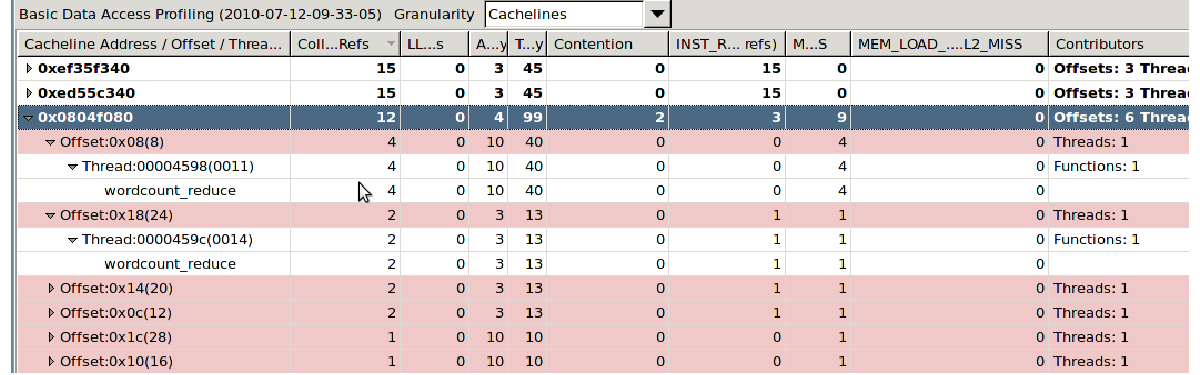
\includegraphics[width=6in]{sheriff/figure/wordcount}
\caption{PTU output for \texttt{word\_count}.
\label{fig:wordcount}}
\end{figure*}

\subsection{\sheriffdetect{} Performance Overhead}
\label{sec:results-runtime-overhead}

\begin{figure*}[!t]
\centering
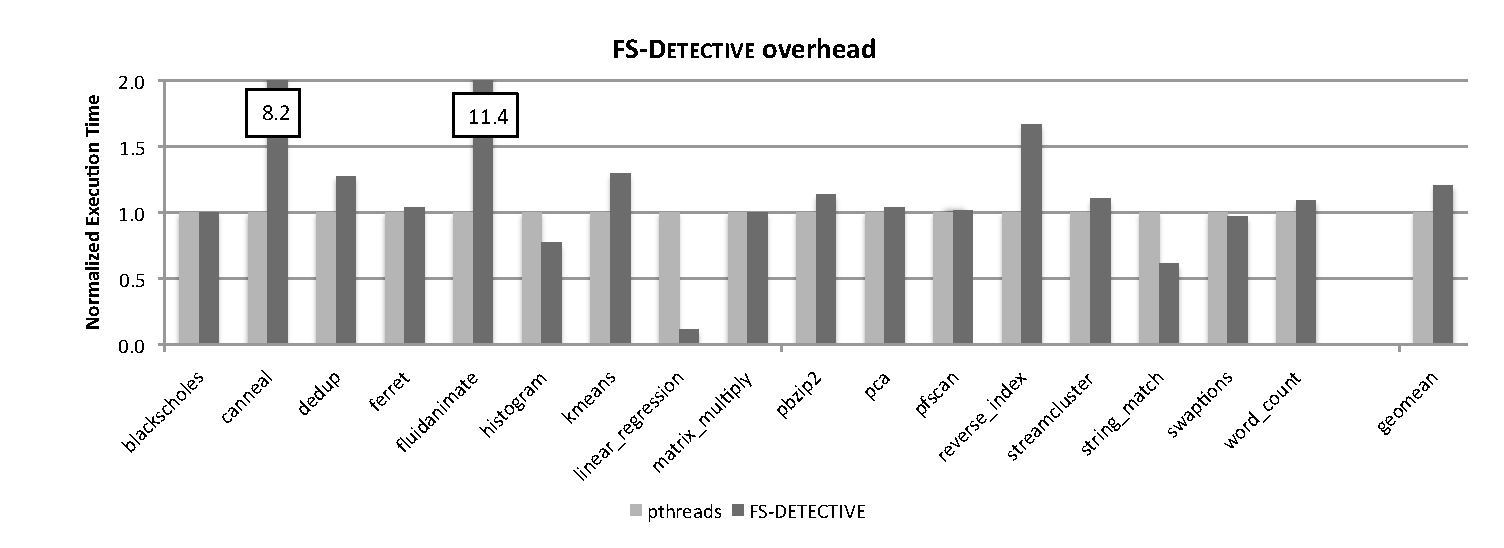
\includegraphics[width=6in]{sheriff/figure/detectiveperf.pdf}
\caption{\sheriffdetect{} performance overhead across two suites of benchmarks, normalized to the runtime of using the \pthreads{} library (lower is better). \label{fig:overhead}}
\end{figure*}


\SheriffDetect{}'s  runtime overhead (comparing to \pthreads{}) on two multithreaded benchmarks suites, Phoenix and PARSEC is shown in Figure~\ref{fig:overhead}.  \SheriffDetect{} only introduces 20\% performance on average, with the exception of three outliers. For other benchmarks, \SheriffDetect{}’s overhead is generally acceptable and far lower than most previous tools.

\texttt{linear\_regression} exhibits almost
a $10\times$ speedup against the one using \pthreads{} library even with the added overhead of sampling and 
other mechanisms of \sheriffdetect{}.  There is a
serious false sharing problem inside (see
Table~\ref{table:perfafterfix}) which both \sheriffdetect{} and \sheriffprotect{} eliminate automatically. 

There are two benchmarks on which \sheriffdetect{} do not perform well. One is \texttt{canneal}, the performance overhead of \sheriffdetect{} on this benchmark is about $7\times$ slower than that using \pthreads{} library. Another one is \texttt{fluidanimate}, the performance overhead is about $14\times$ slower than that using \pthreads{}.

According to our analysis, the number of transactions and dirty pages are two main causes of the performance overhead. Usually more transaction number can cause more dirty pages.   

For a dirty page in every transaction, \sheriffdetect{} handles a page fault, creates two additional pages -- a ``working page'' and a ``twin'' page, checks false sharing problems at every sampling interval, and commits those local changes to the shared mapping. Thus, given large amount of dirty pages, copying overhead alone is very expensive and can dominate most of overhead. For example, \texttt{Canneal} invokes around 2.2 million dirty pages, thus leading to substantial overhead. \texttt{fluidanimate} has a large number of lock calls. Since \SheriffDetect{} replaces lock calls with their interprocess variants and triggers a transaction end and begin for each, thus, \texttt{fluidanimate} runs much slower on the \SheriffDetect{} than on the \pthreads{} library.
 
%%%%%%%%%%%%%%%%%%%%%%%%%%%%%%%%%%%%%%%5
%%%% Some data to list the effectiveness of this tool.
%%%%%% How many caches are carried for each test case. 
%%%%%% Whether all caches has false sharing problem.
%%%%%%%%%%%%%%%%%%%%%%%%%%%%%%%%%%%%%%%
\subsection{\SheriffDetect{} Sampling Rate Sensitivity}
\label{sec:results-sampling-overhead}

\SheriffDetect{} employs the sampling mechanism to detect false sharing happening in long-running transactions. Sampling is only triggered when a transaction's runtime exceeds a pre-defined sampling interval, usually 10ms. Inside the timer handler, \SheriffDetect{} tracks memory accesses and updates cache liens status words. Thus, there is a precision-cost tradeoff: increased sampling rates may uncover more false sharing problems, but at the cost of increase performance overhead. 

To measure \sheriffdetect{}'s sensitivity to the sampling rate, we compare its behavior under three different sampling rates: 2ms, 10ms (our baseline), and 50ms.

\paragraph{Sampling Overhead:} Figure~\ref{fig:sensitivity} shows the performance overhead under these different sampling rates, normalized to the runtime of using 10ms sample interval. Generally, the choice of sampling interval has little performance impact across all evaluated benchmarks. For most of these benchmarks, sampling imposes relatively
small overhead.

One outlier is \texttt{canneal}, which is extremely sensitive to the sampling rate.  When the sampling interval is 2ms, \texttt{canneal} runs about $2.3\times$ slower than that with  the 10ms sampling interval. Also, \texttt{canneal} runs 35\% slower with the 50ms sampling interval than that with the 10ms
sampling interval. The reason is that \texttt{canneal} dirties a large number of shared pages. More frequent sampling thus increases the amount of checking overhead.


\begin{figure*}[!t]
\centering
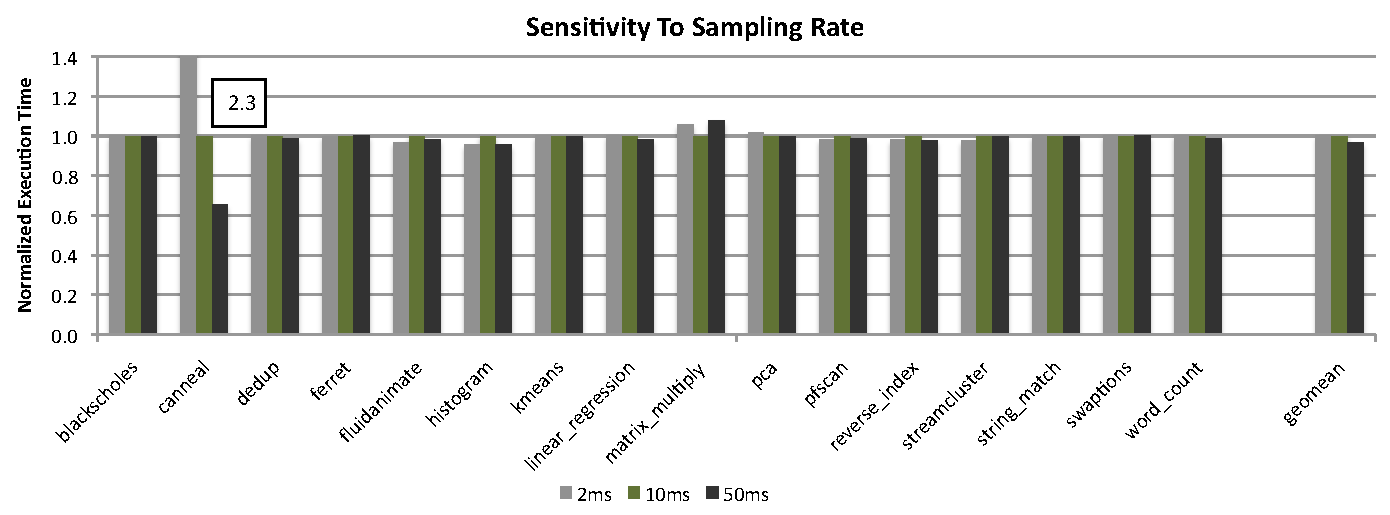
\includegraphics[width=5in]{sheriff/figure/sensitivity}
\caption{\sheriffdetect{} performance with different sampling rates,  normalized to the performance with a sampling interval of 10ms (presented in Figure~\ref{fig:overhead}); lower is better.
\label{fig:sensitivity}}
\end{figure*}

\begin{table*}[!t]
\centering
\resizebox{\columnwidth}{!}{
\begin{tabular}{l|rr|rr|rr}
\hline
{\bf \small Benchmark} & \multicolumn{2}{c|} {\bf \small 2ms} & \multicolumn{2}{c|} {\bf \small 10ms}& \multicolumn{2}{c} {\bf \small 50ms}\\
& {\em objs}  & {\em writes} & {\em objs}  & {\em writes} & {\em objs}  & {\em writes} \\
\hline
\small \texttt{canneal} & 1 & 21444321 & 1 & 26369324 & 1 & 30580451 \\
\small \texttt{ferret} & 1 & 3 & 0 & 0 & 0 & 0 \\
\small \texttt{fluidanimate} & 1 & 3370 & 1 & 4064 & 1 & 2851 \\
\small \texttt{kmeans} & 2 & 2974 & 2 & 1122 & 1 & 98 \\
\small \texttt{linear\_regression} & 1 & 1050 & 1 & 311 & 1 & 71 \\
\small \texttt{reverse\_index} & 5 & 14494 & 5 & 14782 & 5 & 14981 \\
\small \texttt{streamcluster} & 2 & 52462 & 1 & 52283 & 1 & 52420 \\
\small \texttt{word\_count} & 4 & 9849 & 4 & 2699 & 3 & 622 \\
\hline
\end{tabular}
}
\caption{
\sheriffdetect{} precision with different sampling rates, including the number of falsely-shared objects and interleaved writes. We omit those benchmarks with no observed cases of false sharing.
\label{table:samplingquality}}
\end{table*}

\paragraph{Sampling Effectiveness:}
The choice of sampling rates has relatively little impact on detection and ranking, as Table~\ref{table:samplingquality} shows. As anticipated, in most cases, the number of falsely-shared objects reported and the number of interleaved writes observed is not significantly different.

While changing the sampling rate affects the number of falsely-shared objects detected, it has little impact on the detection results for falsely-shared objects with a significant performance impact. For example, increasing the sampling rate to 2ms reveals two additional falsely-shared objects (for \texttt{ferret} and \texttt{streamcluster}), but the number of additional interleavings is quite low (under 10 for those objects). Similarly, reducing the sampling rate to 50ms results in the detection of two fewer objects overall (\texttt{kmeans} and \texttt{word\_count}), but these objects have little impact on performance.


\subsection{\SheriffProtect{} Performance Overhead}
\label{sec:results-runtime-overhead}

\begin{figure*}[!t]
\centering
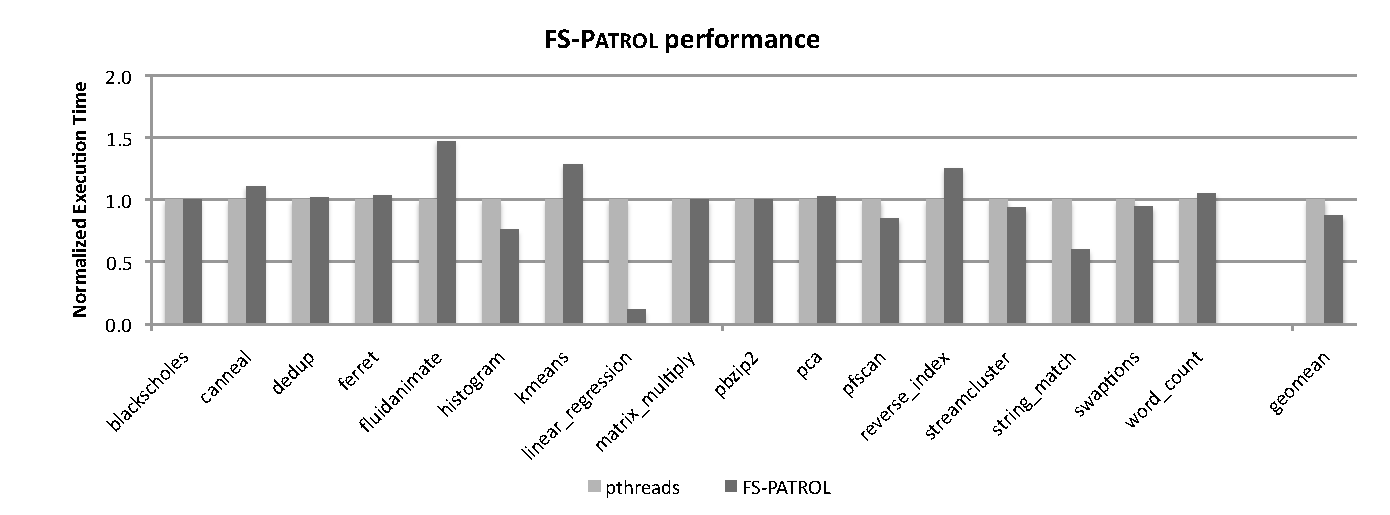
\includegraphics[width=5in]{sheriff/figure/patrolperf.pdf}
\caption{\sheriffprotect{} performance across two suites of benchmarks, normalized to the performance of the \pthreads{} library (see Section~\ref{sec:results-runtime-overhead}). In case of catastrophic false sharing, \sheriffdetect{} dramatically increases performance.
\label{fig:patrol}}
\end{figure*}

Here, we examine the performance improvement by tolerating the false sharing problems in \sheriffprotect{}, which is shown in Figure~\ref{fig:patrol}.  

From the results, we can see that \texttt{linear\_regression} exhibits almost a $10\times$ speedup against the one using \pthreads{} library. By tolerating the serious false sharing problem inside (see Table~\ref{table:perfafterfix}), \sheriffprotect{} achieves a significant performance benefit for this benchmark.

There are three benchmarks which runs at most 30\% slower than using the \pthreads{}. We examine the reasons to cause this slowdown. For \texttt{kmeans}, this application creates more than 3000 threads about 8 seconds. Since the overhead of creating one process is higher than that of creating one thread, this part of overhead dominates most of overhead. 

For \texttt{reverse\_index} and \texttt{fluidanimate}, 
they exhibit slowdown because of the use of the processes-as-threads framework. This performance impact arises from the use of a file-based mapping, which connects the private mapping and shared mapping. The Linux page fault handler does more work when operating on file-based pages than on anonymous pages (the normal status of heap-allocated pages). The first write on a file-mapped page repopulates information from the file's page table entry. Also, the shared store for all heap pages is initially set to \texttt{MAP\_SHARED}, so writing to one shared page can cause a Copy-On-Write operation in the kernel even when there is only one user. 

\texttt{fluidanimate} has an enormous number of transactions(18 Million), \sheriffprotect{} 
introduces some additional overhead for every transaction. That also accounts for part of
overhead.
